\begin{otherlanguage*}{brazil}

\section{Playsound}

O desenvolvimento da plataforma Playsound.space começou durante o meu período de estágion o Centre for Digital Music (C4DM) na Queen Mary University of London (QMUL)\footnote{O Estágio aconteceu de junho de 2017 a maio de 2018 e foi financiado pelo Programa de Doutorado Sanduíche da CAPES}, onde tive a oportunidade de participar do grupo de pesquisa ligado ao projeto Audio Commons\cite{Font2016}. Depois de desenvolver o projeto Banda Aberta, o desejo era de trabalhar no desenvolvimento de um sistema que pudesse ser utilizado como um instrumento musical, que fosse capaz de produzir uma gama rica de sonoridades e não mais somente uma plataforma para tocar sons pré determinados. 

A iniciativa Audio Commons visa trazer conteúdo sonoro em Creative Commons (CC) para artistas e indústrias criativas. Licenças CC fornecem uma maneira padronizada para dar permissão ao público no compartilhamento e utilização de trabalho criativo em condições definidas pelos criadores de conteúdo, que pesquisa formas de aproveitamento e utilização de serviços online de distribuição de conteúdo sonoro com licenças em Creative Commons footnote{\url{https://creativecommons.org/}}. O projeto é financiado pela união Européia e tem entre seus obetivos, desenvolver uam ontologia para sons, e criar um mecanismo mediador para pesquisar sons de diversas fontes como as bilbiotecas Freesound.org, um grande repositório de samples; Europeana.org, que reúne um acervo de gravações históricas de diversas intituições européias e Jamendo.com, que reúne músicas novas produzidas em licensas livres.


Nosso principal domínio de aplicação é a improvisação musical que é definida como uma atividade musical autônoma \cite{Canonne2016} que geralmente leva a situações pluralistas, com ênfase no processo de tocar, e na iteração musical no momento \cite{BERGSTROEM-NIELSEN2016}. Em oposição à improvisação idiomática, como aquela praticada em algumas formas de jazz ou hip-hop, a improvisação livre pode levar à formas não metrificadas e sem escala ou tonalidade pré-determinadas, onde muitas vezes a variação de timbre prevalece\cite{Barthet:11a}. Já vinha desenvolvendo atividades em improvisação livre anteriormente, mas depois do início do doutorado, tive oportunidade de participar da Orquestra Errante, grupo conduzido pelo professor Rogério Costa que ensaia semanalmente no estúdio do NuSom na Universidade de São Paulo. 

Durante as práticas de improvisação musical que participei até agora, encontrava algumas dificuldades em utilizar softwares tradicionais como DAW patchers. Uma delas é de que muitos softwares do tipo DAW são baseados em grids temporais fixos, ou seja, existe um tempo que determina o fluxo dos acontecimentos sonoros, e embora esse tempo possa ser mudado, a estrutura rígida conflita com a necessidade da liberdade na improvisação. A estrutura em grade ou se impõe para os demais músicos, como um metrônomo, ou entra em conflito com os demais participantes. Além disso, as estruturas temporais também dificultam a criação de polirritmias. 

Softwares que se comportam como instrumentos virtuais, por outro lado, como sintetizadores e \emph{samplers} são mais fáceis de serem empregados na prática. Por serem baseados em gesto, o controle do fluxo sonoro fica a cargo do musicista, dependendo aí do tipo de controlador que ele usa, de sua expertise técnica em tocar, e da capacidade de variação timbrística do instrumento. No caso dos sintetizadores, as possibilidades de variação de sonoridade são constringidas pelos timbres oferecidos pelo fabricante ou programador, e em geral restritas a sons musicais, dentro de uma escala pré-determinada. Além disso, para se obter um bom controle de dinâmica, é recomendado a utilização de controladores externos, como teclados midi, por exemplo. Minha idéia era desenvolver algo que pudesse ser tocado em tempo real, e que permitisse mais variação sonora do que os softwares e ferramentas disponíveis no mercado.

No Contexto de novas interfaces para produção musical uma série de abordagens diferente têm sido desenvolvidas para o emprego do computador como instrumento musical na prática de improvisação livre. Exemplos incluem \emph{live coding} \cite{freeman2011collaborative} e orquestras de laptop \cite{Albert2012}. \emph{Live Coding} colaborativo ao vivo frequentemente envolve o desenvolvimento de tecnologia pra sincronização entre dispositivos \cite{Wilson2014}, que aqui não foi adotada devido à escolha estética de deixar a estrutura rítmica livre.


A ideia de tocar com uma ``paleta de sons expandida'' tem sido explorada na música desde Luigi Russolo  \cite{Merz2013} e especialmente depois da música concreta. A digitalização e a disponibilização de sons online potencializa essa ideia, como aponta Schnell:
\begin{citacao}
``In the age of digital sound databases and online music publishing services, the total disembodiment of digital sound turns into the promise of perpetual reincarnation of digital sounds through their permanent exchange and transformation."\cite{Schnell2013}
\end{citacao}

Nos instrumentos que funcionam a base de amostras de sons (samplers), as possibilidades sonoras são ampliadas pela possibilidade de utilização de sons não-musicais, ou em outras escalas, mas são dependes de se ter acesso e conhecimento de uma biblioteca grande de sons. Localizar samples em tempo real durante uma improvisação musical pode ser desafiador\cite{Xambo2018}, principalmente porque a improvisação exige do musicista uma reação espontânea e instantânea em tempo real \cite{canonne2011model}. Isso exige que o performer conheça bem e previamente os sons de uma determinada coleção, o que se torna impraticável se a coleção de sons é muito grande. Para contornar este problema, os praticantes normalmente selecionam uma amostra reduzida de sons, o que acaba também por reduzir suas possibilidades criativas durante as performances.

A digitalização do som, em conjunto com tecnologias Web e bancos de dados de áudio digital abre muitas possibilidades critativas, que como Schnell aponta, pode levar à ``promessa de reencarnação perp´tua de sons digitais através da sua permanete troca e transformação'' \cite{Schnell2013}. A utilização de amostras de sons pré-gravados é largamente empregada em uma série de tradições estéticas musicais como no emph{Hip Hop, Plunderphonics, Música Eletrônica, Música Concreta, composição de Paisagens Sonoras}. Bibliotecas online de áudio como Freesound.org, Redpanal.org, Sampleswap.org entre outras são utilizadas por compositores e produtores musicais de vários tipos de aplicações multimídia como cinema, publicidade, video games, e composições musicais \cite{Roma2013}. 

Alguns projetos desenvolvidos recentemente têm também esse norte como paradigma. O projeto API Cultor, por exemplo \cite{Ordiales2017} usa técnicas de \emph{machine learning} para prover um ambiente para re-utilização de sons de blibliotecas online. Lee et al. propõe uma ferramenta para \emph{live coding} com a API do Youtube para improvisação livre \cite{Lee}. Ao prover acesso a seu banco de dados por uma REST API \cite{Akkermans2011}, o site Freesound.org permite que musicistas e designers criem aplicativos que explorem seu conteúdo online para utilização ao vivo. BeatPush \cite{Feenstra2016}, é um exemplo de sequenciador usando esta API e o Freesound Explorer \cite{Font2016}, por exemplo, organiza os sons em uma configuração espacial por similaridade e usa cores para representar aspectos timbrais, no entanto, é uma aplicação mais voltada para navegação e exploração do que para tocar em tempo real, e não permite que os usuários selecionem sons a partir de buscas múltiplas. 


Entre diversos serviços que provém conteúdo sonoro online, uma imensa gama de sons musicais e não musicais são oferecidos pelo Audio Commons Ecossystem \cite{Font2015}. A ideia no desenvolvimento do Playsound era de ser uma tentativa de contornar essas questões, promovendo o acesso a esses sons em tempo real através da API do Freesound \cite{Akkermans2011}, oferecendo feedback visual através de espectrográficos, de uma forma que pusesse ser tocada sem um grid de tempo fixo e por usuários sem domínio de técnicas musicais.

Compor a partir de espectrogramas era uma idéia que acompanhava meu trabalho já faz algum tempo. Em 2011 publiquei um trabalho chamado UTOPIA, onde desenhava a palavra utopia através de síntese subtrativa sobre uma gravação feita de uma serra de fita em funcionamento, que era uma amostra bastante saturada. Essa idéia também voltou outras vezes no meu trabalho, na composição da peça Bandas Críticas e no processo de composição de sons para o Banda Aberta. Quando começamos a publicar os primeiros artigos a respeito do projeto Banda Aberta comecei a buscar ferramentas para conseguir imprimir os conjuntos de samples (ver figuras \ref{samplesgalaxias}, \ref{samplespercussao}, \ref{samplescolab} e \ref{samplesorquestra}) e não consegui encontrar nenhuma ferramenta pronta que pudesse gerar espectrogramas de um conjunto grande de sons que fosse acessível, então para gerar essas imagens, bem como os sites que reúnem os samples do projeto, precisamos desenvolver uma ferramenta própria, que chamamos de spectrogram player, que foi o esboço de um player a partir de spectrogramas, em JavaScript e HTML \footnote{A ferramenta foi desenvolvida em código aberto e está disponível no endereço: \url{https://github.com/arianestolfi/spectrogramplayer}}. Quando comecei a desenvolver este novo projeto, descobri que a API do Freesound já fornecia os spectrogramas dos sons de sua bilbioteca, o que era muito conveniente para o projeto, já que diminui o tempo necessário para a análise via FFT que poderia gerar os spectrogramas em tempo real. Além disso, ao oferecer os spectrogramas como imagens, a API do Freesound permite realizar a pesquisa sonora sem a necessidade de baxar os sons toda vez no computador do usuário.

Além disso, queria desenvolver uma ferramenta que não dependesse de expertise técnica ou virtuosismo, que é um dos objetivos dessa pesquisa. Assim como no projeto Banda Aberta, decidioms manter o texto como forma de interação com o sistema, mas ao invés de fazer um mapeamento de sons por letras, como no projeto anterior, aqui o texto serve como fonte para buscar informações, ao permitir a busca através de significados semânticos ou descritivos, por exemplo: ``chuva pacífica'', ``crowd noise'' ou ``raucous cockatoos''. A solução técnica foi o desenvolvimento de um sistema de busca que provém o acesso a centenas de milhares de sons em Creative Commons baseada na API do Freesound.

\subsection{Motivações}




\subsection{Desenvolvimento do Projeto}


\begin{figure}
\centering
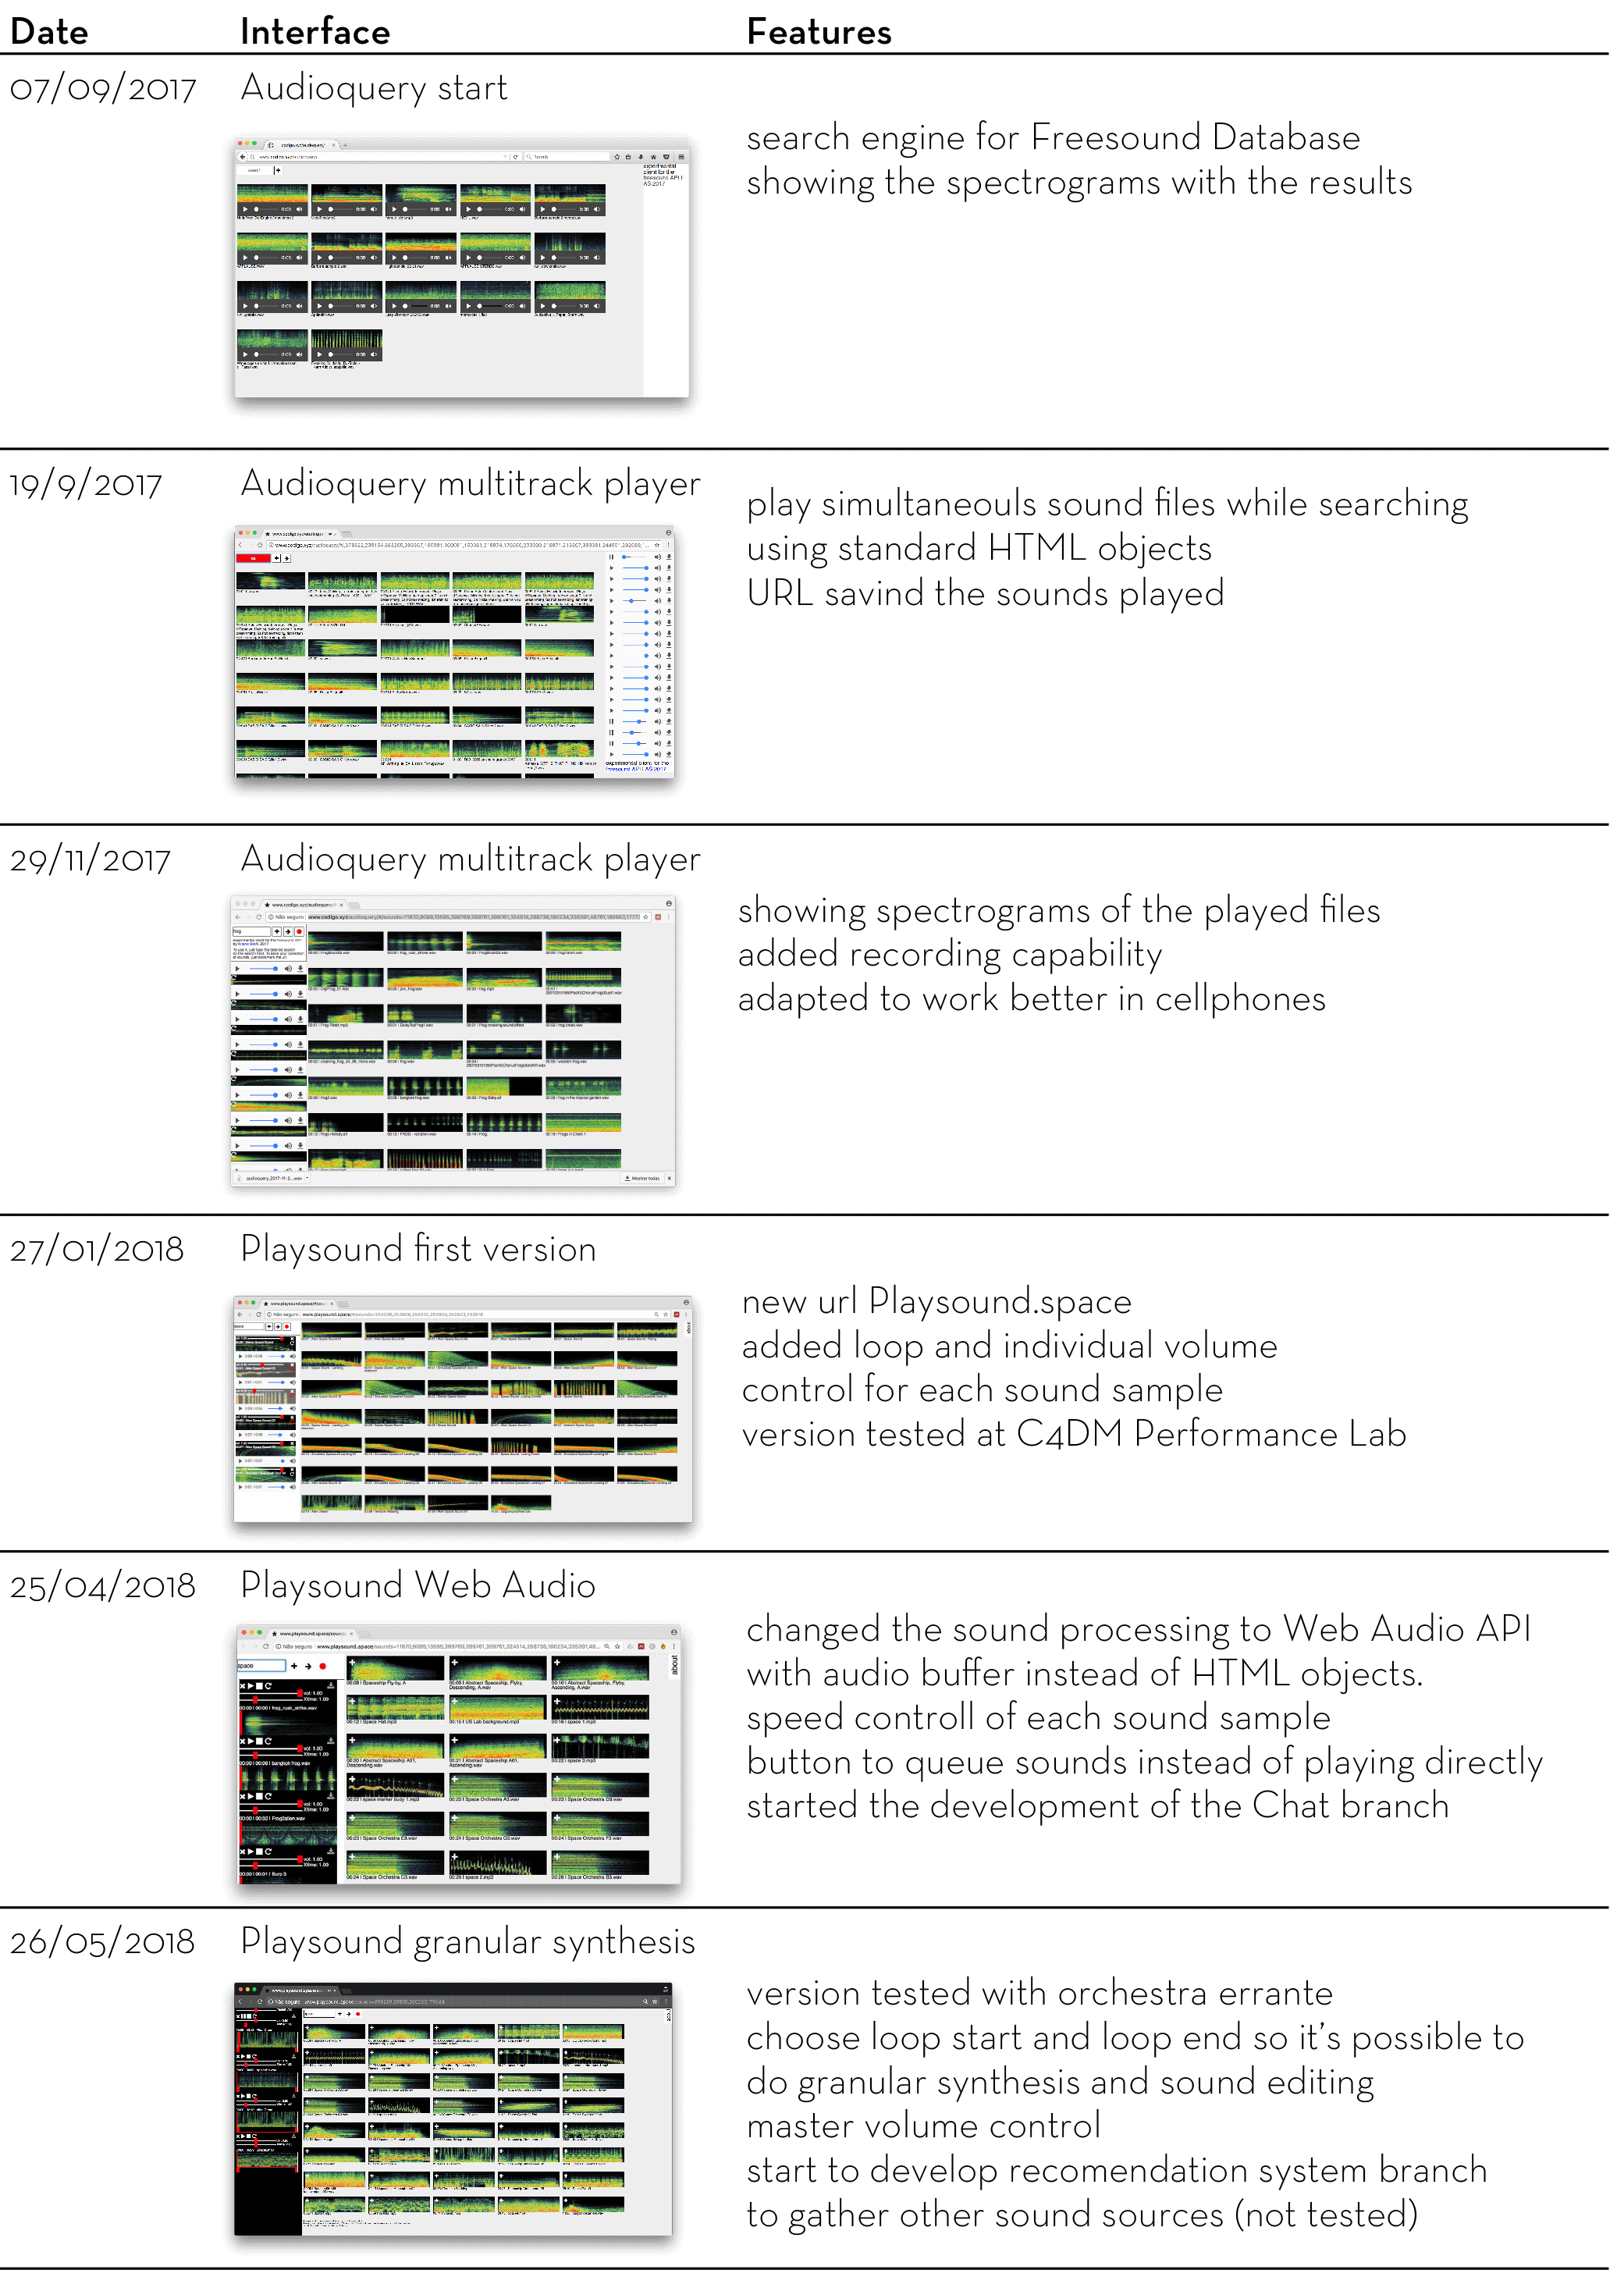
\includegraphics[width=0.8\textwidth]{pictures/playsoundtimeline}
\caption{\label{pstimeline}Playsound development timeline}
\label{fig:timeline}
\end{figure}

Comecei a desenvolver o projeto em Julho de 2018, após apresntar o Banda Aberta em alguns eventos na Europa que descrevi na seção anterior. A figura \ref{fig:timeline} apresenta os principais estágios de desenvolvimento da ferramenta de Setembro de 2017 a Julho de 2018. Utilizei novamente Lean Ux \cite{Liikkanen2014} como metodologia de desenvolvimento de software. Dentro dos princípios desse método, começamos novamente o projeto a partir de um protótipo bem simples, que era apenas um sistema de busca que mostrava o resultado como um conjunto de spectrogramas. Inicialmente, contei com a ajuda do programador Miguel Ceriani para fazer a ligação com a API do freesound.

Utilizamos como \emph{framework} Angular.js\footnote{Angular.js é um \emph{framework} em JavaScript desenvolvido pela Google que permite automatizar certos processos computacionais e facilita a comunicação com bancos de dados}. O Framework fornece o recurso de ligação de dados bidirecional, que faz com que a busca aconteça no servidor simultaneamente ao se digitar o texto na caixa de busca. Deste modo, mesmo antes de se completar uma palavra, resultados já começam a aparecer na janela do navegador. Para o processo de improvisação livre, esse recurso se mostrou muito interessante, uma vez que sons não esperados podem surgir mesmo antes de se estabelecer um vocábulo definitivo. 

Os resultados são apresentados na forma de spectrogramas, que permitem que o usuário do sistema tenha informações sobre ritmo e timbre das amostras recebidas antes de escolher o som para tocar. Os resultados são apresentados em uma matriz, que permite que se compare os sons visualmente. Apesar de a leitura dos spectrogramas não ser uma coisa corriqueira para qualquer usuário do sistema, acreditamos que um aprendizado implícito pode acontecer no simples processo de pesquisar e tocar com o sistema, quando se percebe a co-relação entre a representação gráfica das propriedades espectro-temporais dos dos sons e suas qualidades audíveis. Quando selecionamos uma imagem, o som é adicionado a uma playlist na lateral da interface.

 Assim que colocamos o sistema no ar, começamos a desenvolver recursos adicionais para transformar o sistema em um instrumento musical de fato. O primeiro recurso desenvolvido foi a capacidade de se fazer novas buscas enquanto os sons são tocados, recurso que já não existe no próprio Freesound. Em seguida, criamos um sistema de url para armazernar uma coleção de sons feita previamente. Cada som selecionado gera um código que fica registrado no endereço do navegador. Desta forma, é possível recuperar uma ``composição de sons'' para utilização futura. O próximp passo foi desenvolver a interface para tocar os arquivos. A primeira versão funcionava baseada em objetos HTML, utilizando o \emph{player} padrão dos navegadores para objetos de áudio que oferece controles apenas de pausar tocar, alterar o instante tocado e dependendo do navedagor um controle de volume. Em uma segunda versão utilizamos o tocador do Freesound, que oferecia recursos de loop, mas isso exigia que se recarregasse a página, interrompendo o fluxo musical. 

 Desenvolvemos alguns recursos básicos do tocador, adicionando a imagem do espectro sonoro como recurso mneumônico, e adicionamos controle individual de volume e loop para cada som que era adicionado à playlist. Como recurso de usabilidade, para dar feedback visual, a transparência da imagem é alterada conforme o volume do som aumenta ou abaixa. Adicionamos também um gravador embutido no sistema, que permite que as seções sejam gravadas em arquivos WAV. Esses arquivos podem ser salvos ou re-inseridos na interface para serem tocados. A figura \ref{fig:audioquery} mostra a interface da primeira versão do software no Google Chrome. \footnote{Por questões acadêmicas, mantemos ainda uma versão funcional do software em \url{http://www.codigo.xyz/audioquery/#/sounds=49333,415849}}.

\begin{figure}
\centering
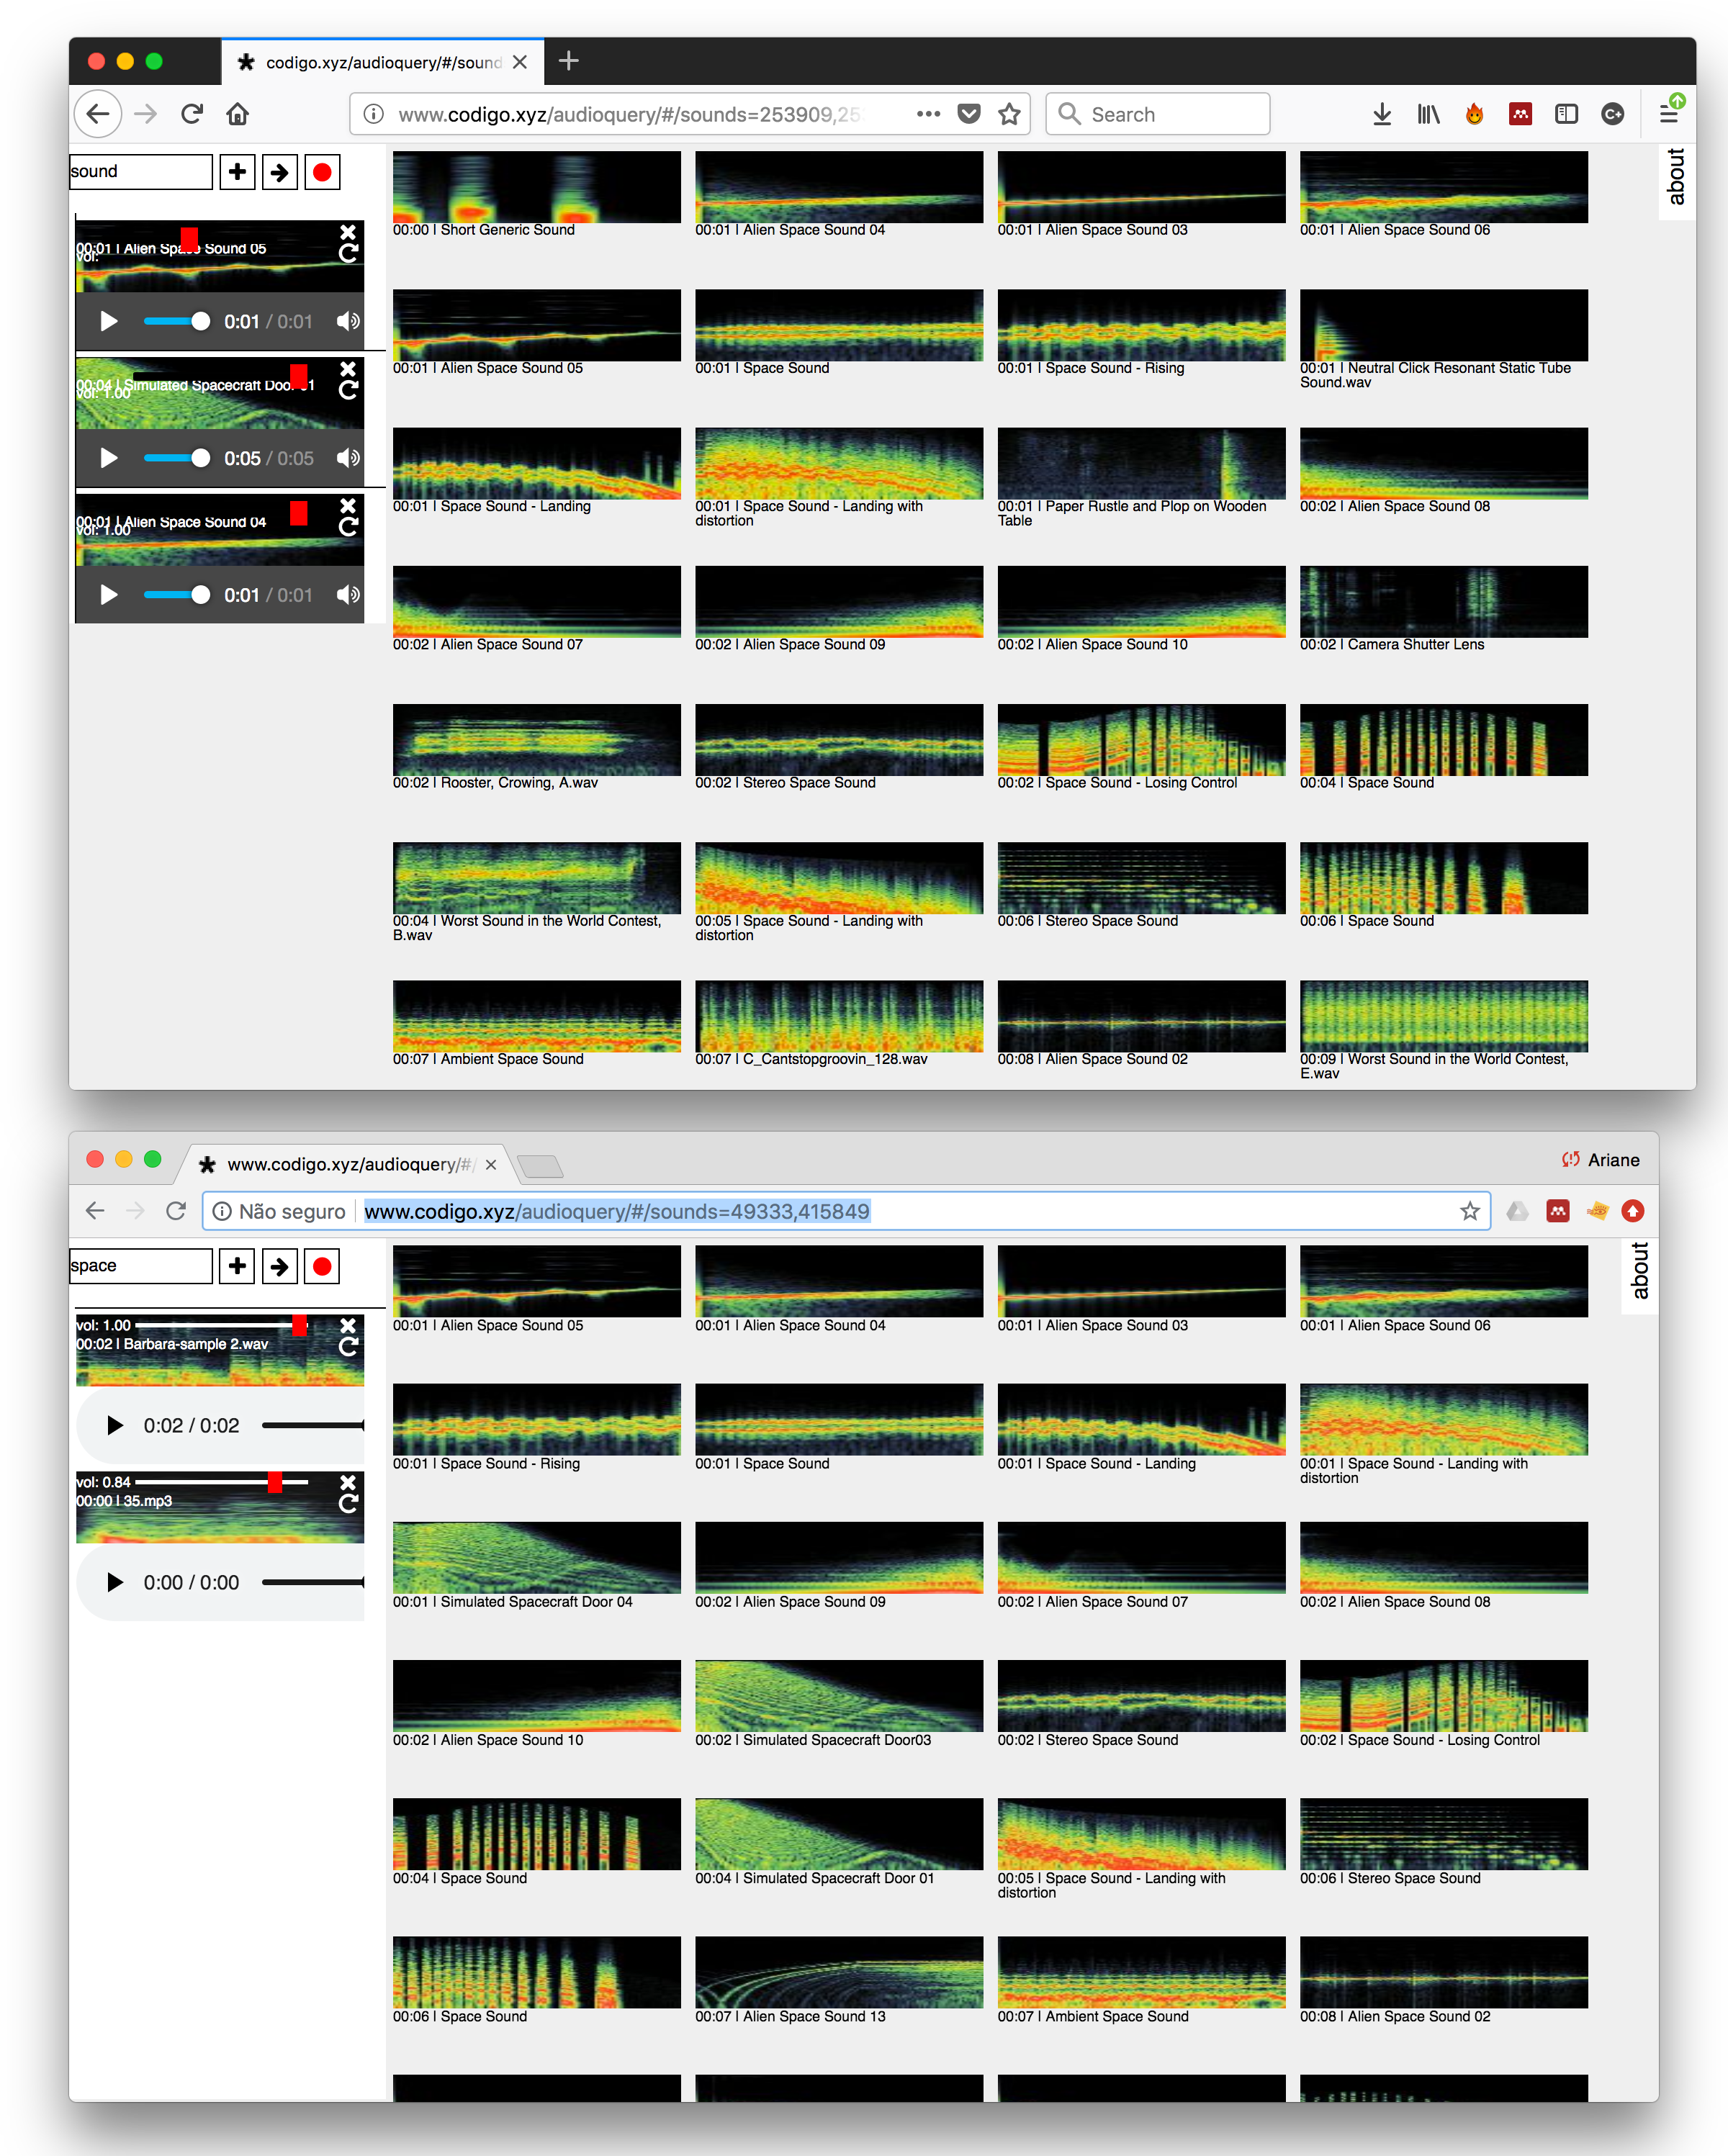
\includegraphics[width=0.8\textwidth]{pictures/cap4/audioquery_browsers}
\caption{\label{audiquery}Primeira versão funcional do software desenvolvida.}
\label{fig:audioquery}
\end{figure}

Durante esta primeira fase, as avaiações foram feitas principalmente pela autora, mas também contando com a opinião de alguns colegas convidados para testar informalmente a ferramenta. Esses testes fora de condições de laboratório são previstos  
 %Mais adiante, passei a contar com a ajuda da {}programadora Alessia Millo, que colaborou no desenvolvimento do tocador e de outros recursos que implantamos no sistema. Ela trabalhou na adaptação do sistema para utilizar as tecnologias de Web Audio, ao invés dos objetos HTML, que permitiu uma série de recursos que implementamos posteriormente, como a possibilidade de escolher o começo e o fim dos pontos de loop, alterar a velocidade de reprodução de sons e posição estéreo dos sons.

\subsection{Primeiras avaliações}

When the system was judged ready to be used in live performances (Audioquery multitrack player in Figure \ref{fig:timeline}), we conducted several user evaluations \cite{Stolfi2018b}. First, we established a small ensemble including musicians playing PS and other musicians playing electronic or traditional instruments such as guitar and effects, piano, percussions, and vocals. In each session, participants were invited to play together an improvisation piece for about 10 minutes, and to discuss their experience after each piece. We examined three sessions with this kind of ensemble, involving 6 musicians in total. Following this study, we improved the interface to provide individual volume control and information about the audio file on the playlist.\footnote{Audio recordings of seven 10 min improvisation pieces are available at the link:\url{http://finetanks.com/records/puppets/}}

In another evaluation, PS was tested in controlled lab settings with trios of participants both with and without prior music performance experience. Participants were invited to play three five-minute long free improvisations using the system on their laptops. 15 participants took part in the study (5 females, 10 males, mean$\pm$SD age = 32.7$\pm$5.4), 8 of them considered themselves as musicians (4 intermediate and 4 experienced), while 7 did not. We measured system usability \cite{Jordan1996} and creativity support \cite{Cherry2014} using an online survey to be completed just after the performances. We also conducted inductive thematic analyses \cite{Braun2006} from focus group discussions and self-reports related to workflow, hedonic quality, engagement, learning, contexts of use and improvements. The prototype yielded a high usability score (M = 82.5/100, SD = 8.94) and creativity support index (M =71.7, SD =15.6) with no significant differences between non musicians and musicians.

The system proved to be inclusive with respect to musical expertise since it enabled creative musical collaborations without training and for users who did not have prior musical skills. We identified design challenges like a will for more control of audio processing (e.g. volume, loop, effects, timing) and increased sense of identification and co-presence between performers. To improve sound retrieval, participants wished to have access to filtering and clustering techniques and to be able to search for sounds by features, e.g. by timbre.

These initial user evaluations were followed by a first live solo performance with PS by the first author at the A'mas event held at the Total Refreshment Centre in London on 25 March 2017 \footnote{Excerpt from the performance can be found at \url{https://youtu.be/LmjmpQagBG8}}. After a 30 minutes solo performance, the performer also joined a jam session with 8 other invited musicians who played synthesizers and other electronic instruments. During the jam, most of the instruments were connected trough a central Midi clock providing beat synchronization. Although PS does not offer this possibility, since it is not grid-based, it was still possible to play live in this format. The performer had to develop a strategy to select in real time sounds that wouldn't conflict with the established rhythm, working with sonic materials such as textures and effects instead of more structured loops. By using this system as part of a public live electronic performance, we acknowledged that it could be used as a basis for real music practice. But as in previous evaluations, the performer also found that the creative control would benefit from enriched audio processing.

\subsection{Melhorias}

Following users' desire for more expressive control, we added a range of audio editing, processing and mixing capabilities. This included the possibility of queuing sounds in the playlist and manipulating their duration and pitch by varying their playback speed. We also enabled editing by selecting segments and control custom loops during playback. To implement this feature, we used the buffer object from the Web Audio API library which replaced the HTML media element object (despite the HTML media object can start playing upon selection large files while still buffering). We also introduced a panning control for each sound object, allowing to position them in the stereo field. We are planning to introduce a panning control on the master channel e.g. to help musicians from laptop ensembles to identify individual sonic contributions spatially.

\subsection{Evaluation with Orquestra Errante Improvisation Ensemble}




\subsubsection{Analysis of the performances}

Audition of the recordings showed that, comparing to the previous tests, most performers from the improvisation ensemble chose to work with fewer sonic materials and spend more time at exploring sound processing instead of using large amount of sound samples. This may be due to the richer amount of expressive controls present in the updated interface, but also a will to closely work with sonorities, which is characteristic of FMI. The performed pieces present a great degree of variation in dynamics and textures, depending on the group configurations. There were interesting musical dialogues between the performers, with question-response situations and different ground-figure relations between PS and traditional instruments. At times, PS players produced accompanying textures and in other occasions, they acted as soloists, as commonly takes place in the practice of the ensemble.


\subsubsection{Thematic analysis}

We conducted a thematic analysis \cite{Braun2006} on the transcriptions of the group discussion and answers to the survey. We identified the recurrent themes below which were also present in the previous analysis \cite{Stolfi2018b}.

\textbf{Creativity support and narrative.} (10 occurrences) Users commented about the process of playing together (\textit{``the sound you played directly influenced on what I was doing, and the inverse also happened"}, \textit{``I've changed the velocity based on what you were playing"}), and about the type of sounds played (\textit{``there were some interesting sounds out of context that we embraced, but sometimes it was almost funny"}). 

\textbf{Relevance and excitement.} (7 occurrences) Some users showed excitement to play with the tool (\textit{``can we play!?"}, \textit{``there's every sound in the universe!"}, \textit{``it's well resolved in terms of sound"}).

\textbf{Emotional engagement and playing strategies.} (10 occurrences) Users reported about the novelty of the tool which provided a different way to play (\textit{``this generates a specific way of playing"}, \textit{``there are interesting sound samples you can manipulate like a sound object"}, \textit{``the nice thing here is the search through words"}), and about how they used the tool during the performances (\textit{``I was playing, then I changed the tempo, then I started to select excerpts of the samples"}).

\textbf{Limitations.} (9 occurrences) Users reported some issues with the current interface, that had misleading controllers and lack of visual feedback about the sounds being played. During the study, the interface faced a bug preventing the playhead positions to show the current position in each audio sample. Participants also commented on the speed of the response, since the Internet speed was very slow during the test.

\textbf{Identification of sounds and sources.} (3 occurrences) Users reported that they were able to listen to the digital sounds. One participant reported the difficulty to know who was playing what, and another suggested that the performance would be better if everyone had their own pair of speakers.

\textbf{Improvements.} Users suggested some desirable improvements such as: including capabilities for time stretching, synchronization of all sounds, to stop all sounds, to use a midi controller, to have a fade in/out options for each sound, and interface with other hardware (e.g. Arduino, Raspberry Pi).

In the survey question on what they most enjoyed using PS, users reported on the quantity of sounds available and empowerment (\textit{``I felt a kind of power to have available a huge quantity of sounds to use"}), and about the possibility of combining \textit{``textures with superimposed layers''}. About the type of sounds used, they reported searching for \textit{``Non-musical sounds"} and \textit{``Low pitched sounds, from the nature"}. One of them interestingly reported \textit{``I didn't search for anything, the sound came to my encounter."}.

\section{New Directions}

Since the last evaluation, we have included new features which will be the object of future evaluations. These features have been developed mostly to enhance participatory processes, by providing a chat environment, and accessibility, through a built-in translation system aiming to let non-English speakers use the tool.

\subsection{Chat}
At the address \url{http://www.playsound.space/chat}, the user can type messages that are shared with other users connected to the same address. Moreover, the messages, once sent, become hyperlinks which, when selected, trigger a query in the Freesound database. This in return shows results for the related word. 

The chat is based on socket communication, implemented in node.js through socket.io. Ids are assigned automatically to the clients accessing the address, and we are currently implementing the creation of user-defined chatrooms.

\subsection{Translation}

Freesound APIs \footnote{https://www.freesound.org/docs/api/overview.html} propose a text search mechanism that operates by matching tags and other metadata. This simple mechanism (exploited by PS) does not account for mismatches between the language that users employ in their queries and the ones used in tagged Freesound content. As this can impair the inclusion of non-english speakers, it motivated us to implement a translation tool, which now allows the user to select its own language and receive possible translations to English, the main language of the metadata. 

Playsound's translation tool relies on Yandex APIs\footnote{\url{https://tech.yandex.com/translate/}}, that supports 90 languages. To simplify the interface, we reduced the range to 17 languages that are more present on Freesound. When users type in a keyword in the research field, PS issues a request to the translate API and propose the results to the users. They are then allowed to click on the suggestion to start the research with the English keyword.

To illustrate how the translation tool can be useful for a user we provide an example based on the Portuguese word \textit{``pandeiro"} (i.e. tambourine in English). At the time of writing, Freesound hosts 52 sounds matching the word ``pandeiro". If Portuguese is set as the input language, PS translation let users query sounds with the English translation of the word, which yields 460 results.

\subsection{Tag and Audio Content-based Recommendation}

Another feature which we develop in parallel provides recommendations of audio files that sound similar to selected ones \cite{Viola2018}. This contribution is framed within the EU-funded Audio Commons project that aims at easing the access to Creative Commons audio content to the creative industries. The implemented recommendation mechanism is a complex multi-agent system based on the Semantic Web of Things. It operates through a two-stages approach: in the first stage it looks for audio files with the same tags on Freesound as well as on Europeana and Jamendo (all these three are content providers of the Audio Commons Ecosystem). In the second stage, an audio analysis is performed to reject results that differ too much from the originally selected file (at the moment a simple similarity function is implemented using spectral linear centroid computed with Sonic Annotator and Vamp plugins \cite{Cannam2010}).

\section{Discussion}

There are currently three instances of Playsound that are developed in parallel. The main instance can be used as a single user instrument or composition tool. The version including the chat system will be developed to become a fully participatory music making tool. The Playsound recommendation system should include in the future sounds from other resources and be integrated into the other instances upon positive result from testing. While some of the features developed came from necessities identified among the test users, other features followed design choices discussed by the authors to better support inclusion (for example the translation system) and to provide access to the Audio Commons Ecosystem (recommendations). Even though tests were made with different users during different phases of development, the core of the analysis mostly comes from the author's continuous practice with the system itself. Eventually, we realized that although porting the system to Web Audio buffers may offer more support in music processing, it also makes the system loose part of its real-time playing capabilities, as currently sound buffers need to be fully loaded before playing.




Numa segunda oportunidade, o professor Leonardo trouxe uma série de playlists com diferentes tipos de sons como glissandos, batidas para realizar uma atividade de preparação de corpo sonoro com a turma de alunos. Um dos alunos operou com facilidade essas playlist improvisando com os sons reúnidos enquanto o professor coordenava a atividade de corpo. 

Mais adiante no curso, quando partimos para produção musical, passamos a utilizar outras ferramentas como editores de áudio e trackers com sintetizadores e samplers. Nesta fase, usamos o Playsound principalmente para pesquisar sons para serem adicionados aos projetos dos alunos, que foram montados posteriormentes nos sequenciadores. Essa breve experiência foi importante para testar vários potenciais de aplicação do Playsound também na esfera educacional. Por ser livre, aberto e sem a necessidade de instalação, é uma ferramenta versátil que pode ser adotada por educadores em diversas práticas.


\begin{figure}[htb]
\label{audiqueryminipage}
\centering
 \begin{minipage}{0.49\textwidth}
   \centering
   \caption{Primeira versão da interface do software} \label{fig_minipage_imagem1}
   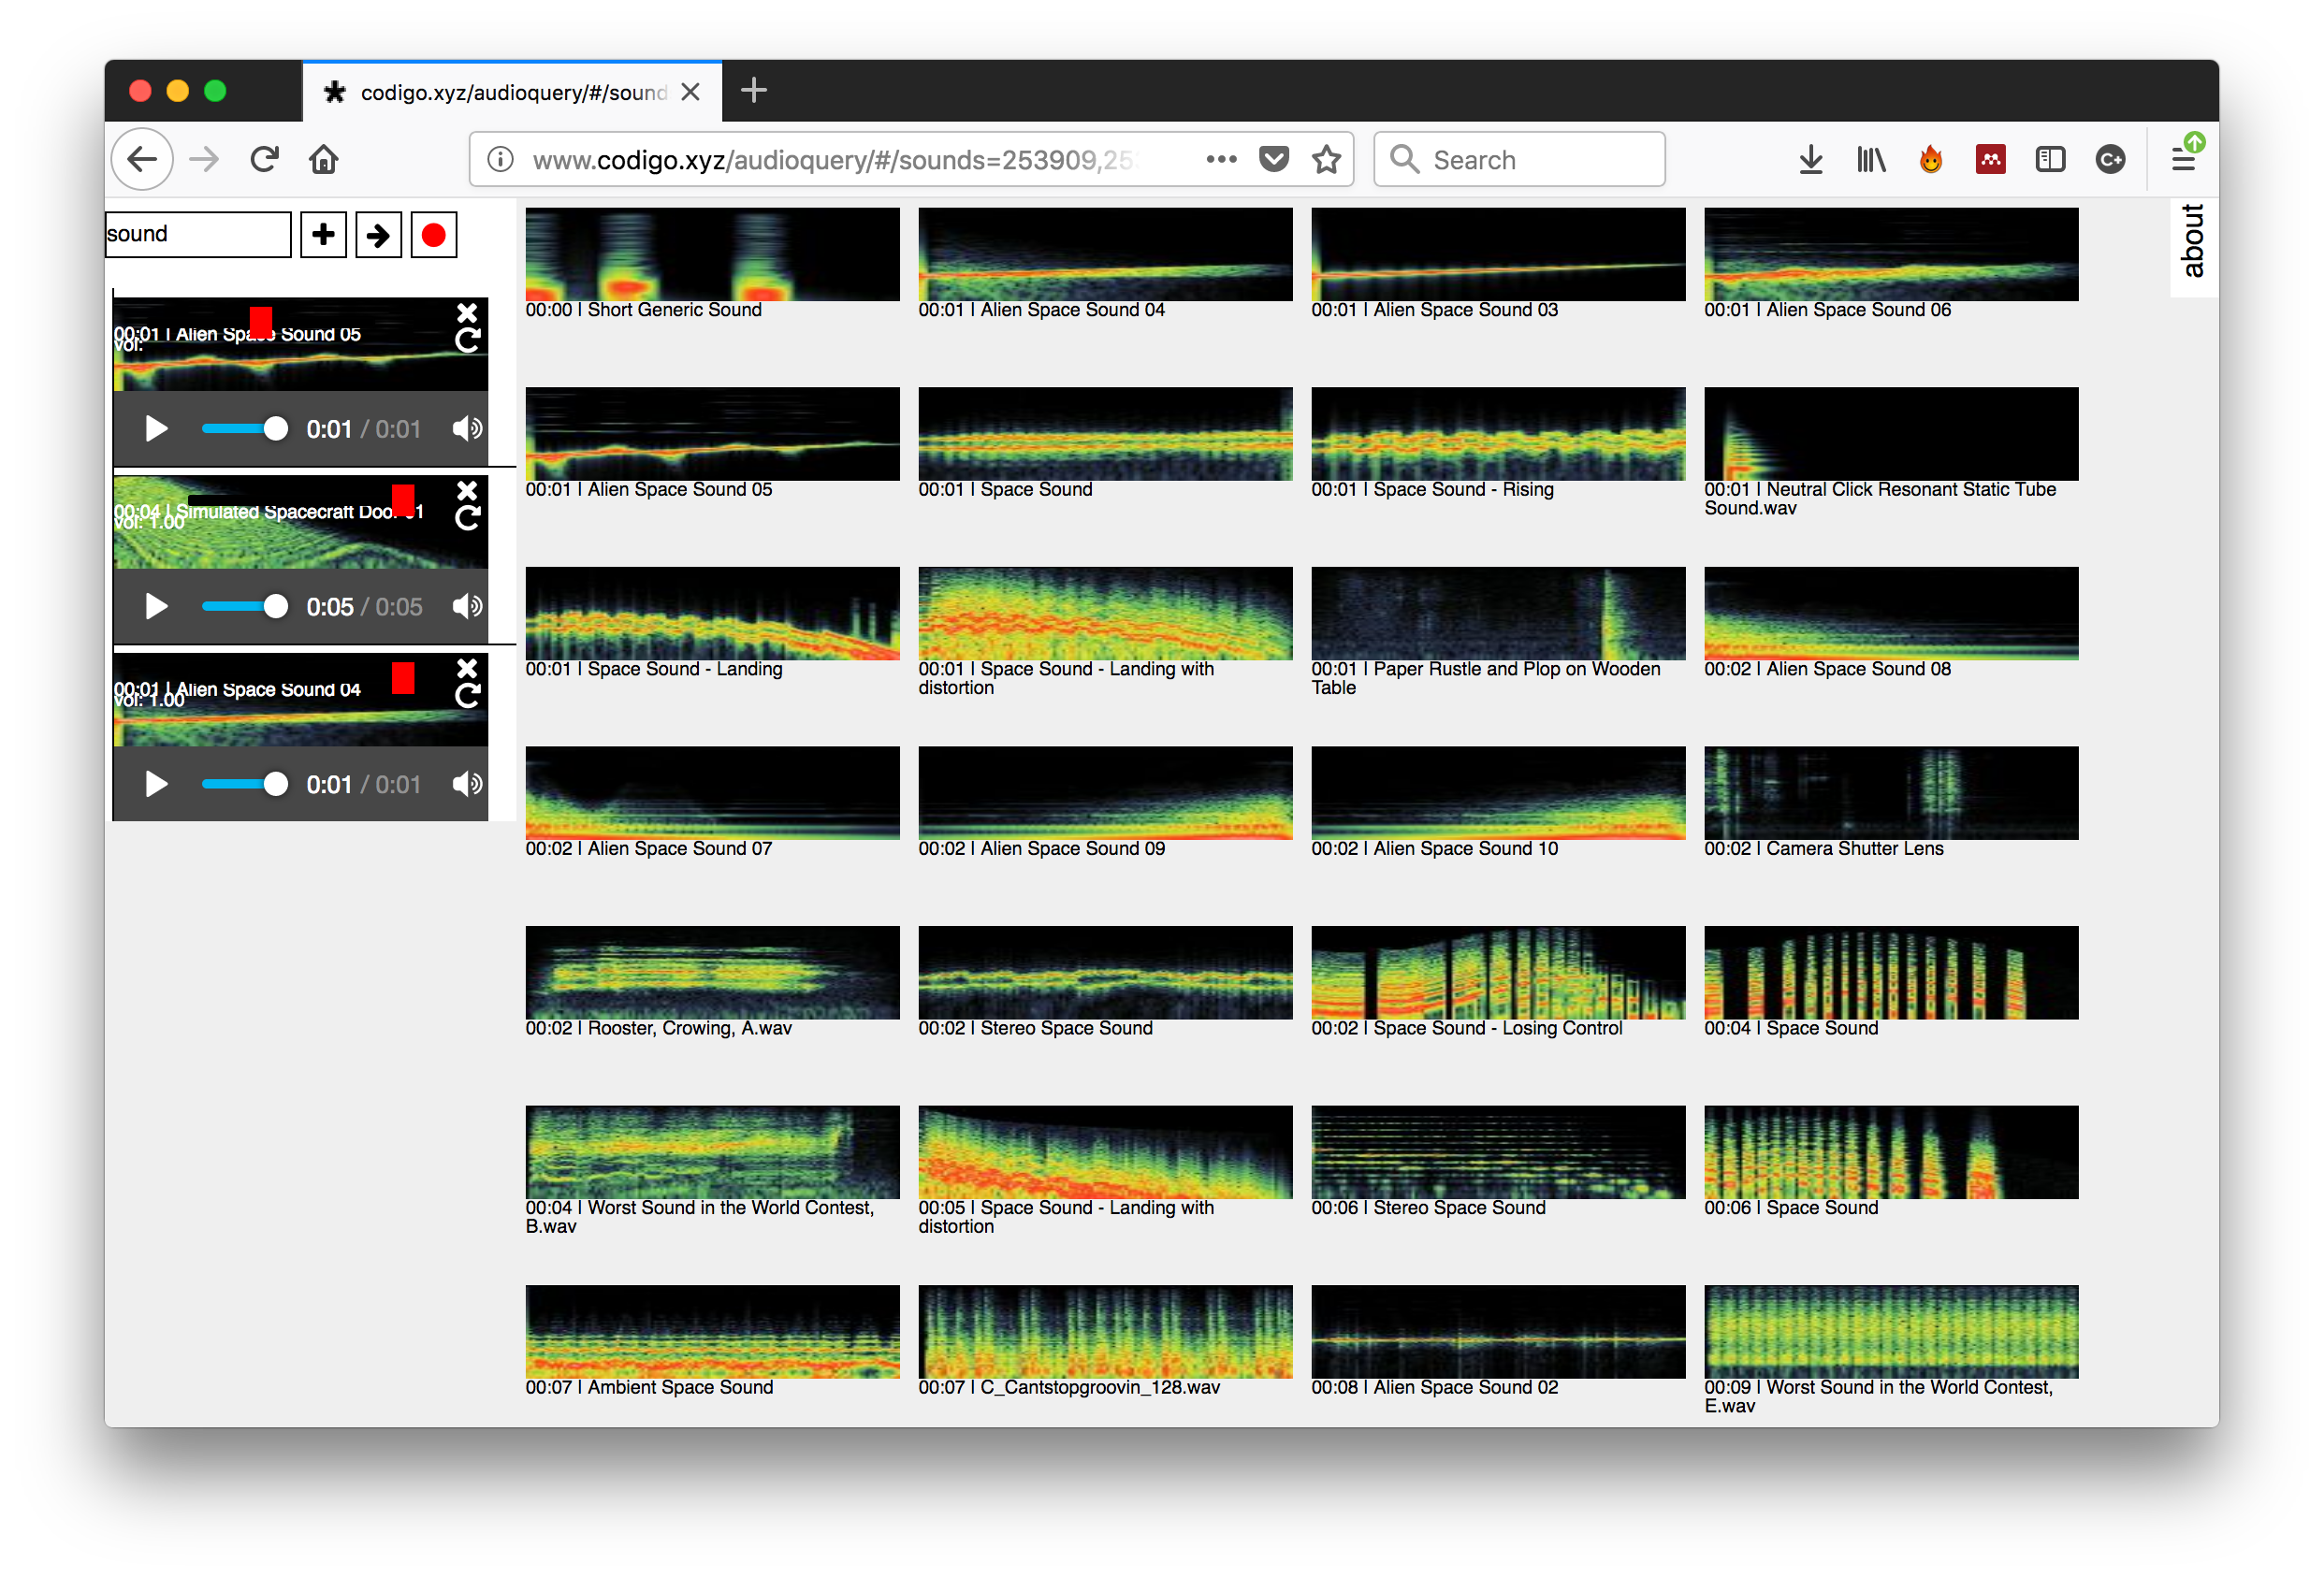
\includegraphics[width=\textwidth]{pictures/cap4/audioquery_firefox}
   \legend{Fonte: Screenshot da autora no navegador Chrome}
 \end{minipage}
 \hfill
 \begin{minipage}{0.49\textwidth}
   \centering
   \caption{} \label{fig_minipage_grafico2}
   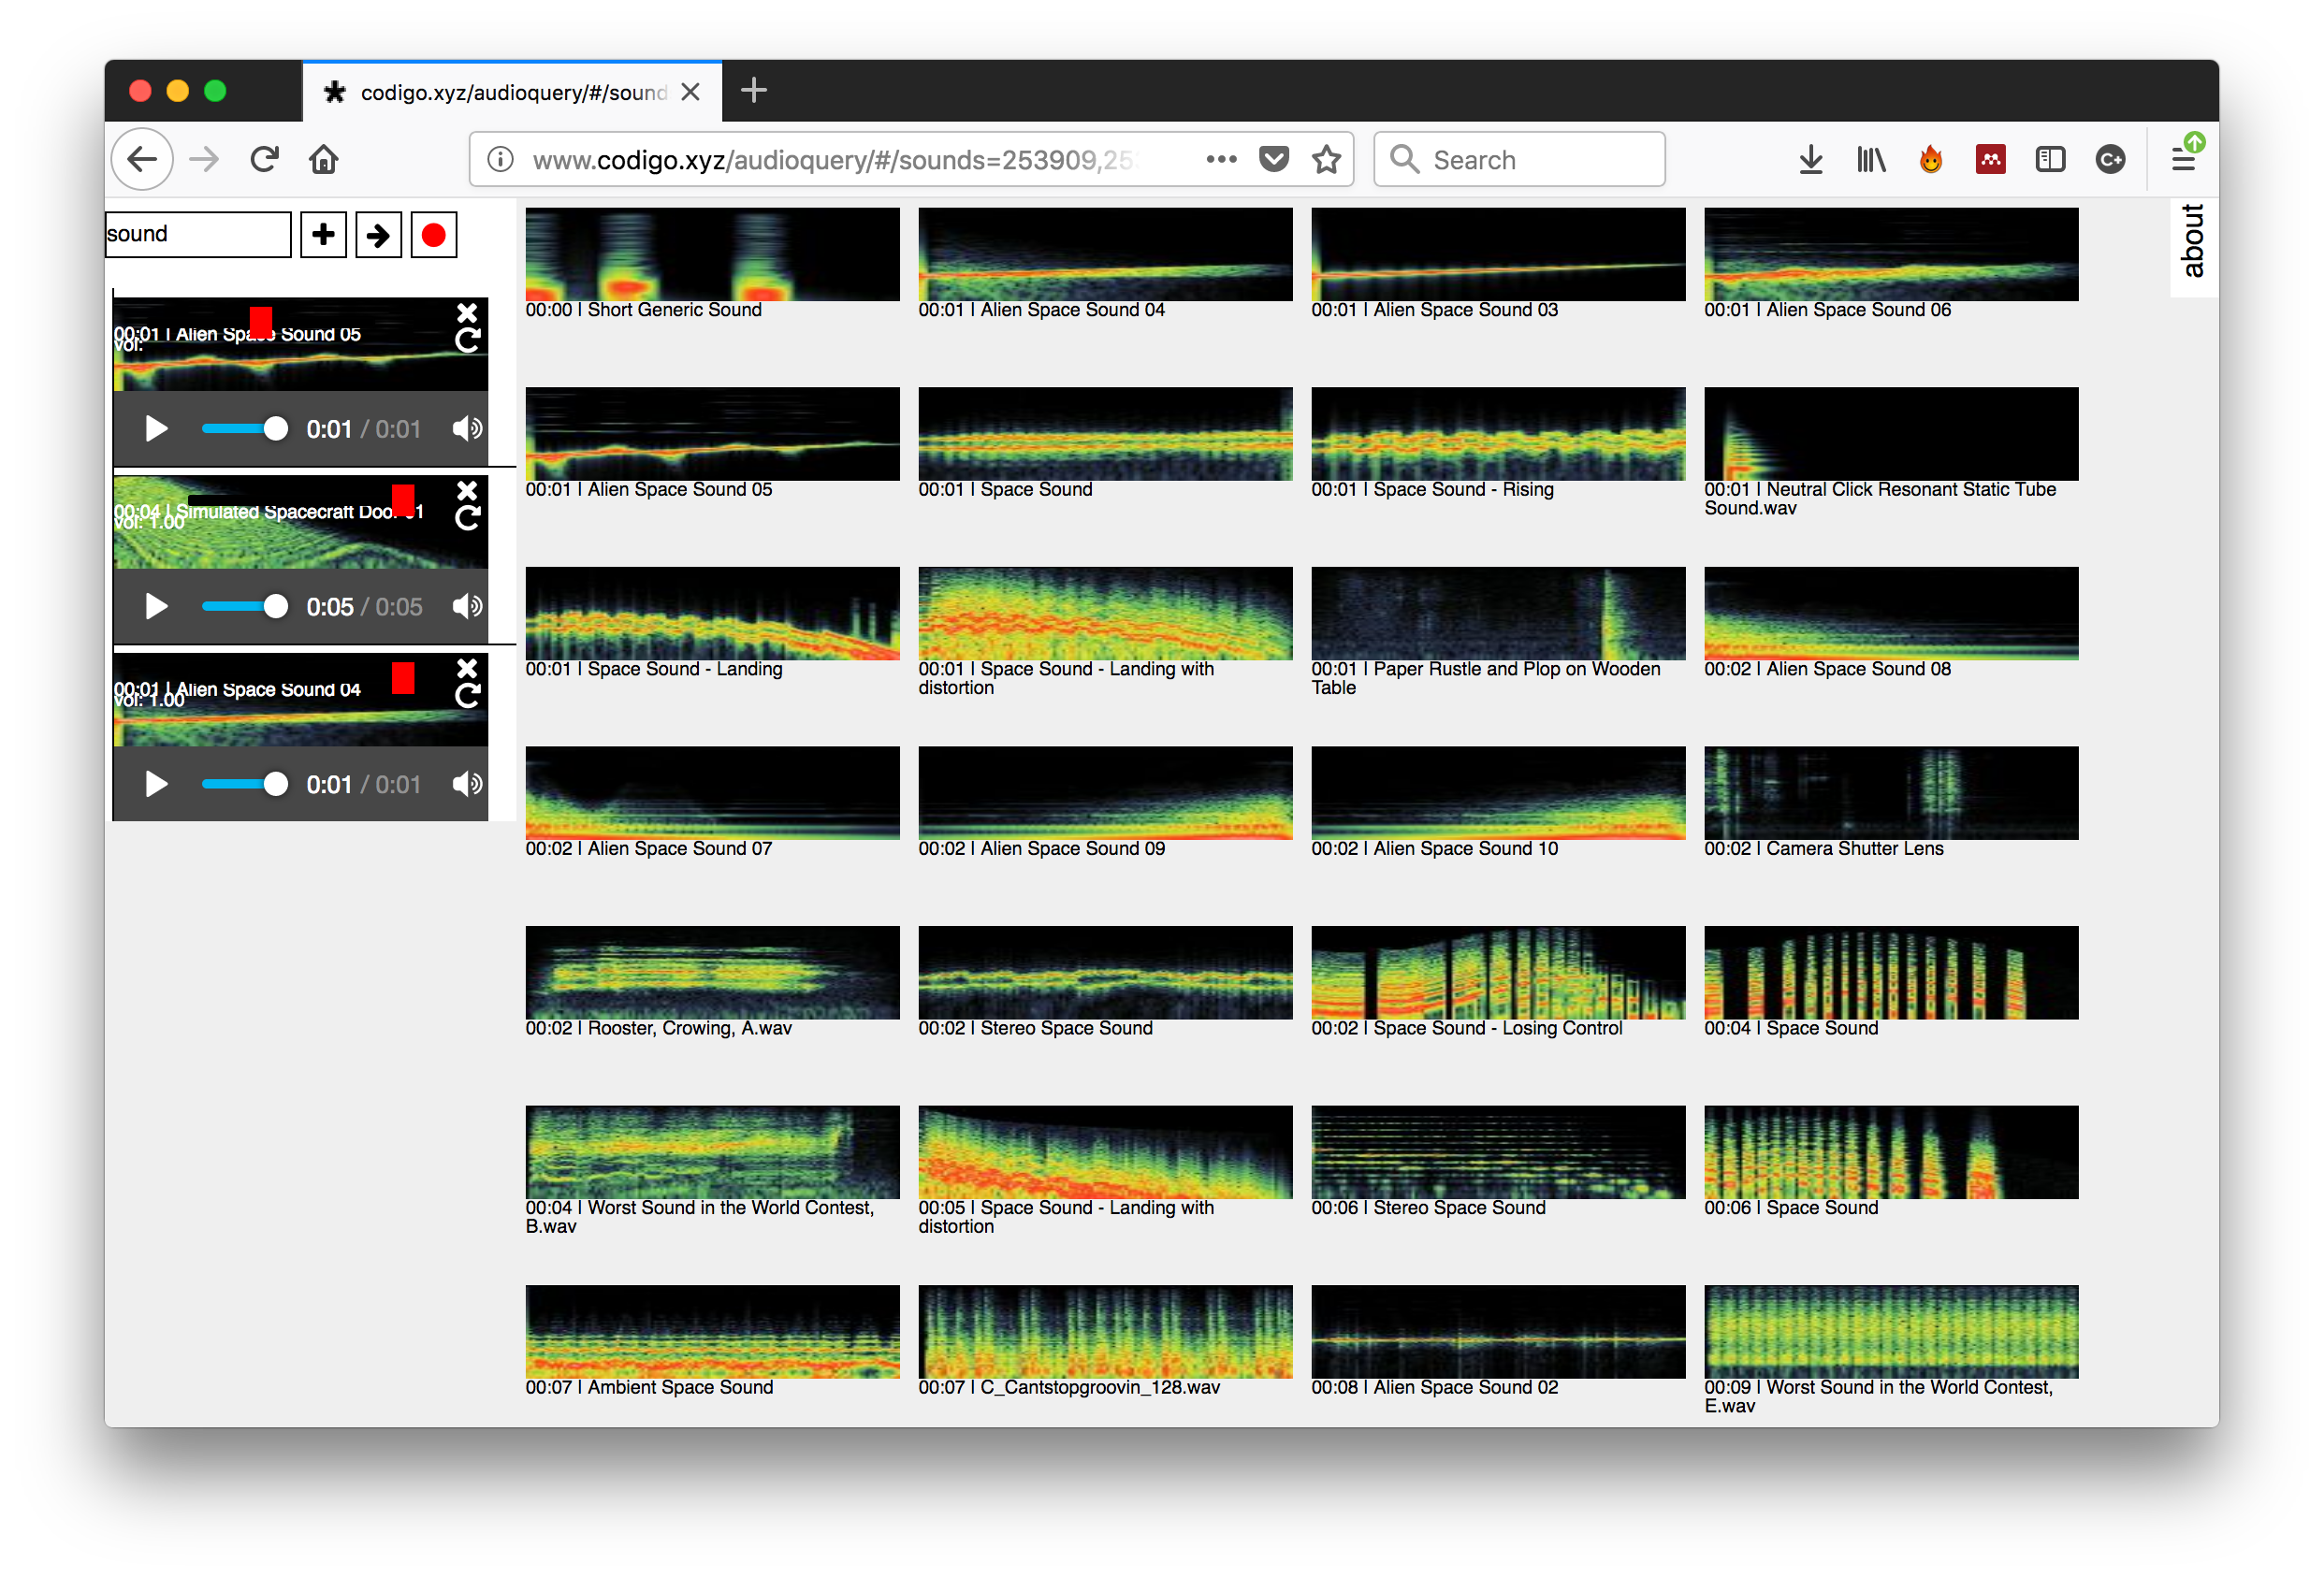
\includegraphics[width=\textwidth]{pictures/cap4/audioquery_firefox}
   \legend{Fonte: Screenshot no navegador Firefox}
 \end{minipage}
\end{figure}


\end{otherlanguage*}

\phantomsection

